\documentclass[a4paper,11pt]{style-esi/td}

\usepackage{style-esi/licence}
\usepackage{style-esi/exercice}
\usepackage{style-esi/exemple}
\usepackage{style-esi/question}
\usepackage{style-esi/tutoriel}
\usepackage{style-esi/listing}
\usepackage{style-esi/images}
\usepackage{style-dev1/dev1}

\begin{document}

\seance{1}{Introduction}
\entete
\titre
\ccbysa{esi-dev1-list@he2b.be}
\lastedit

\bigskip
\tableofcontents

\vfill
%\newpage
\begin{coltbox}{Conseils}
	Quelques conseils pour bien travailler et progresser.
	\begin{itemize}
	\item 
		Faites bien tous les exercices proposés.
	\item 
		Vous pouvez \textbf{coopérer} avec vos condisciples 
		mais nous vous demandons de ne \textbf{pas copier} les réponses. 
		Si vous voulez progresser, \textbf{chercher} la réponse est plus important que de la trouver. 
	\item 
		N'hésitez pas à \textbf{montrer votre travail} à votre professeur.
	\item 
		N'hésitez pas à \textbf{poser des questions} 
		si vous n'avez pas bien compris ce qu'on vous demande.
	\item 
		\textbf{Prenez des notes} ! 
		Ce que vous allez apprendre aujourd'hui 
		vous servira les semaines prochaines 
		mais vous en aurez oublié une grande partie si vous ne notez rien. 
		Le plus pratique est probablement d'annoter la version \textbf{papier}. 
	\end{itemize}
\end{coltbox}
\vfill

% \newpage
% %===================
% \section{Windows}
% %====================

% 	Comme vous avez pu le constater, 
% 	les \name{PC} des laboratoires sont équipés du système \name{Windows}.
% 	Au laboratoire d'environnement, vous vous connecterez sur un serveur \name{Linux}. 
% 	\name{Windows} vous servira essentiellement à : vous connecter au \name{Linux}, 
% 	effectuer des recherches sur Internet, imprimer et transférer des fichiers.
% 	Si vous avez une question concernant l'utilisation de Windows 
% 	vous trouverez peut-être la réponse dans l'aide-mémoire disponible sur \name{poÉSI}. 		

% 	%====================
% 	\subsection{S'identifier}
% 	%====================

% 		\begin{infobox}
% 			\begin{description}
% 				\item[Votre login]
% 					est simplement votre numéro d'étudiant.
% 				\item[Votre mot de passe]
% 					vous a été communiqué par mail lors de votre inscription.
% 					C'est le même mot de passe que celui pour vous connecter
% 					à votre mail \name{he2b} ainsi que tous les autres service associés.
% 				\end{description}	
% 		\end{infobox}

% 	%====================
% 	\subsection{Imprimer}
% 	%====================

% 		Si vous voulez imprimer ce \name{TD} (ce qui est une bonne idée), 
% 		vous devez \textit{installer} une imprimante. 
% 		Vous trouverez comment faire en consultant l'aide-mémoire que vous venons de mentionner.
	
% 	%====================
% 	\subsection{Changer le mot de passe sous Windows}
% 	%=====================

% 		\subparagraph{Réflexion.}
% 		À votre avis, pourquoi vous demande-t-on de modifier votre mot de passe ?
					
% 		\begin{Exercice}{Exemples de mots de passe} 		
% 			Quelles sont les propositions qui vous paraissent correctes comme mot de passe ?
% 			\par
% 			\qquad\checkbox~\samp{nadia}
% 			\qquad\checkbox~\samp{M0nAm1eN@di@}
% 			\qquad\checkbox~\samp{m@C0p1ne}
% 			\qquad\checkbox~\samp{GH5).jg}
% 		\end{Exercice} 
	
% 		Il est  temps de \textbf{changer votre mot de passe}. 
% 		Consultez l'aide-mémoire si vous ne savez pas comment faire. 
				
% 		\begin{infotbox}{Règles sur les mots de passe}
% 			Sur les \name{PC} de l'école,
% 			un mot de passe doit comporter au moins 8 caractères
% 			parmi au moins 3 des 4 catégories suivantes : 
% 			minuscules, majuscules, chiffres et autres caractères.
% 		\end{infotbox}

% 		\begin{faq}
% 			\textbf{J'ai oublié mon mot de passe. Qu'est-ce que je peux faire ?}
% 			\par
% 			Les professeurs ne peuvent ni retrouver votre nouveau mot de passe, 
% 			ni remettre le mot de passe de départ. 
% 			Par contre, les techniciens (bureau au 5\ieme) 
% 			peuvent remettre le mot de passe de départ. 
% 			Allez les trouver (et prenez garde à ce que ça n'arrive plus !)
% 		\end{faq}
	
\newpage
%===================
\section{Une introduction à Linux}
%====================

	\exergue{Linux ? Il y a moins bien mais c'est plus cher.}{Auteur inconnu}

	%====================
	\subsection{Présentation}
	%====================

		Vous ne travaillerez pas directement sur votre PC durant les laboratoires d'environnement. 
		Celui-ci vous servira pour vous connecter au serveur Linux
		(son nom est \verb_linux1_).

		\begin{theorie}{Linux}
			\begin{wrapfigure}{r}{0.4\textwidth} 
				\vspace{-1em}
				\flushright
				
\includegraphics[width=0.38\textwidth]{images/ubuntu}
				\caption{Ubuntu 18.04}
				\vspace{-1em}
			\end{wrapfigure} 
			Linux est un système d'exploitation comme le sont également Windows ou MacOS. 
			Il permet d'utiliser l'ordinateur et ses périphériques. 
			La plupart des systèmes d'exploitation actuels proposent 
			une interface graphique à l'utilisateur. 
			Ainsi, les concepts de fenêtre, de menus, de souris\dots{} vous sont familiers. 
			Linux n'échappe pas à la règle et propose un environnement 
			proche de ce qu'on peut trouver sur d'autres systèmes.
		\end{theorie}

		Bien que nous pourrions utiliser le mode graphique, 
		nous allons, pour des raisons pédagogiques, 
		vous apprendre à utiliser Linux en mode console.

		\begin{theorie}{Le mode console}
			\begin{wrapfigure}{r}{0.55\textwidth} 
				\vspace{-1em}
				\flushright
				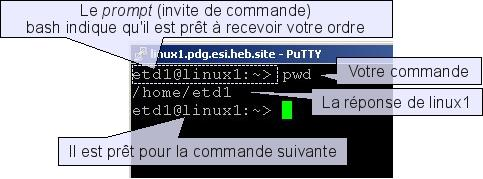
\includegraphics[width=0.53\textwidth]{images/console}
				\vspace{-1em}
			\end{wrapfigure} 
			En mode console%
			\footnote{%
				On parle aussi de mode \og{}commande\fg{} ou encore \og{}terminal\fg{}.
			}, 
			nous n'allons pas utiliser des fenêtres et une souris 
			mais nous allons donner (\textbf{écrire}) des commandes au système.
			\begin{description}
			\item[Shell] 
				Un programme dont le but 
				est d'accepter des commandes de la part de l'utilisateur 
				et de les exécuter. 
				C'est ce shell qui tourne dans la console.
			\item[Bash] 
				Plusieurs shells existent en Linux. Bash est l'un d'entre eux.
			\end{description} 
			Dans l'exemple ci-dessus, 
			vous pouvez constater que l'utilisateur entre la commande \kbd{pwd}  
			qui a pour effet d'afficher une réponse%
			\footnote{%
				Vous comprendrez bientôt ce que signifie \kbd{pwd}.
			}. 
			Ensuite, bash attend la commande suivante.
		\end{theorie}

		Pour travailler en mode console, il faut savoir dialoguer avec ce shell. 
		Comment lui indiquer par exemple qu'on veut copier un fichier, 
		exécuter un programme Java\dots ? 
		\textbf{C'est le principal objectif de ces TDs !}

\newpage
	%====================
	\subsection{Se connecter}
	%=====================

		\verb_linux1_ n'est pas la machine sur laquelle vous êtes.
		Vous allez devoir vous y connecter à distance.

		\begin{theorie}{putty}
			\textbf{\name{putty}} est une application qui permet (notamment)
			d'ouvrir un \emph{terminal} sur une machine distante, 
			de s'y connecter et de dialoguer avec elle en mode console.
		\end{theorie}

		\begin{colxbox}[colback=white,halign=center,drop fuzzy shadow]
		\begin{centering}
			\begin{minipage}{10em}
				\centering
				
\includegraphics[height=6em]{images/putty1}\\
				{\footnotesize Vous, sur le PC Windows}
			\end{minipage}
			\qquad
			\begin{minipage}{8em}
				\centering
				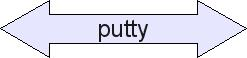
\includegraphics[height=2em]{images/putty2}
			\end{minipage}
			\qquad
			\begin{minipage}{10em}
				\centering
				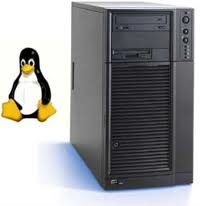
\includegraphics[height=6em]{images/putty3}\\
				{\footnotesize linux1}
			\end{minipage}
		\end{centering}
		\end{colxbox}

		\bigskip
		Lorsque vous allez vous connecter, \verb_linux1_ va vous demander de vous identifier.

		\begin{infobox}
			\begin{description}
			\item[Votre login (username)]
				Un \textbf{'g' minuscule} suivi de votre numéro d'étudiant
				(ex: \samp{g52010}).
				\textbf{Note} : pour Linux, les minuscules et les majuscules 
				sont toujours des caractères différents.
			\item[Votre mot de passe]
				Le même que votre \textbf{mot de passe initial sous Windows}%
				\footnote{%
					Le mot de passe sous Windows,
					sous Linux et pour votre mail \name{he2b} 
					sont trois mots de passe différents
					mais initialisés à la même valeur.        
				}.			
			\end{description}
		\end{infobox}

		\begin{Tutoriel}{Connectez-vous à linux1} 
		Il y a 4 étapes :
		\begin{steps}			
		\item 
			Lancez l'application \name{putty} 
			(vous la trouverez dans le menu ou comme raccourci sur le bureau).			
		\item 
			Indiquez à \name{putty} le nom de la machine (\textit{Host Name}) 
			à laquelle vous voulez vous connecter (ici \kbd{linux1}) ;
		\item 
			Cliquez sur "\textbf{Open}" ; 
			la connexion se fait ! 
			S'il vous présente une boite de message avec un "\textbf{Security Alert}", 
			cliquez sur "\textbf{Yes}" en toute confiance.			
		\item 
			Identifiez-vous !
			\begin{steps}
			\item 
				Tapez votre nom d'utilisateur (cf. plus haut) 
				puis sur la touche \verb_ENTREE_. 
			\item 
				Tapez votre mot de passe (cf. plus haut) puis sur la touche \verb_ENTREE_.
				\par
				\textbf{Note} : Rien ne s'affiche quand vous tapez votre mot de passe ; c'est normal.
			\end{steps}
		\end{steps}
		\end{Tutoriel}

\newpage
	%====================
	\subsection{Le dossier personnel et le dossier courant}
	%=====================

		\begin{theorie}{Fichiers et dossiers}
			Comme sur la plupart des systèmes d'exploitation 
			les données sur le disque dur 
			sont organisées en fichiers et dossiers :
			\begin{itemize}
			\item 
				Un \textbf{fichier} contient de l'information : 
				un code Java, un exécutable, un texte\dots{}
			\item 
				Un \textbf{dossier} contient des fichiers. 
				Il sert à organiser/regrouper les nombreux fichiers du disque. 
				On parle aussi de \textbf{répertoire}.
			\item 
				Un dossier peut aussi contenir des dossiers qui, à leur tour, 
				peuvent contenir des fichiers/dossiers qui\dots{}
				On a une organisation \textbf{hiérarchique} des fichiers.
			\end{itemize}
		\end{theorie}

		\begin{theorie}{Le répertoire personnel}
			Sur Linux, chaque utilisateur dispose d'un « \textbf{dossier personnel} » 
			(on dit aussi sa « \textbf{home} »). 
			C'est dans ce dossier qu'il peut créer des fichiers (et des dossiers). 
			Par convention, ce dossier porte le même nom que le login de l'utilisateur%
			\footnote{%
				À ne pas confondre avec le dossier qui s'appelle \samp{home}
				et qui contient tous les répertoires personnels.
			}.
		\end{theorie}

		\begin{theorie}{Le dossier courant}
			À tout moment,
			on se trouve dans un dossier précis, le \og{}\textbf{dossier courant}\fg{}. 
			Au départ, lorsqu'on se connecte, c’est le \emph{répertoire personnel}.
		\end{theorie}

	%====================
	\subsection{Visualiser le contenu d'un dossier/fichier}
	%=====================

		Commençons notre apprentissage en douceur
		en voyant comment visualiser ce qui se trouve dans notre dossier.

		\begin{Experience}{Visualiser le contenu d'un dossier}
			\vspace{-1em}
			\begin{steps}
			\item 
				Entrez la commande \kbd{ls} (n'oubliez pas la touche \verb|ENTREE|).				
				\begin{Console}
					linux1:~> ls
					dev1 welcome
				\end{Console}				
				Le bash vous montre le contenu de votre dossier courant
				(votre dossier personnel dans ce cas ci).
				Vous constatez qu'il contient déjà un dossier \samp{dev1}
				et un fichier \samp{welcome}.
				Pour vous aider à faire la différence
				entre un dossier en un fichier, 
				la commande \samp{ls}
				affiche les noms de dossiers dans une couleur différente.
			\item 
				Entrez à présent la commande \kbd{ls dev1}.
				\begin{Console}
					linux1:~> ls dev1
					readme
				\end{Console}				
				Cette fois, il vous montre que le dossier \samp{dev1} contient
				un fichier appelé \samp{readme}.
			\end{steps}			
		\end{Experience}

\newpage

		\begin{Experience}{Visualiser le contenu d'un fichier}
			Vous avez vu que votre dossier contient un fichier \samp{welcome}.
			Qu'y est-il écrit ?
			\begin{steps}
			\item 
				Entrez la commande \kbd{cat welcome}.
				\begin{Console}
					linux1:~> cat welcome
					Bienvenue sur la machine linux1 de l'ÉSI.
				\end{Console}
				La commande n'est pas la même pour voir le contenu d'un fichier
				ou d'un dossier.
			\end{steps}			
		\end{Experience}

		\bigskip
		\begin{theorie}{Visualiser le contenu}
			\begin{itemize}
			\item \kbd{ls}
				(sans rien derrière) liste le contenu du dossier courant.
			\item \kbd{ls nomDuDossier}
				liste le contenu du dossier indiqué.
			\item \kbd{cat nomDuFichier}
				affiche à l'écran le contenu du fichier dont le nom est donné 
				(on peut juste le voir, pas le modifier !).
			\end{itemize}
		\end{theorie}
	
	%====================
	\subsection{La structure d'une commande}
	%=====================

		Faisons quelques expériences pour comprendre
		la structure générale d'une commande.

		\begin{Experience}{La casse} 
			\vspace{-1em}
			\begin{steps}
				\item Entrez la commande \kbd{LS} (en majuscule).
			\end{steps}
			Vous voyez que le résultat est différent :
			il vous affiche un message d'erreur 
			car il ne comprend pas ce que vous lui voulez.
			\begin{infobox}
				En Linux, 
				\textbf{les majuscules et les minuscules n'ont pas le même sens.}
			\end{infobox}
		\end{Experience}	
			
		\begin{Experience}{Les espaces} 
			Tapez ces 3 commandes qui ne se différencient 
			que par la présence ou non d'espaces.
			\begin{steps}
			\item \kbd{ls dev1}
			\item \kbd{lsdev1}
			\item \kbd{ls dev 1}
			\end{steps}
			À nouveau le résultat est différent dans les 3 cas. 
			\textbf{Les espaces ont de l'importance}.
		\end{Experience}				

		\begin{theorie}{Une commande décomposée}
			Une commande est composée de plusieurs parties 
			séparées par un ou plusieurs espaces. 
			\begin{center}
				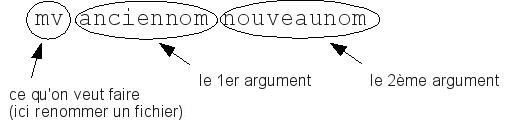
\includegraphics[width=0.6\textwidth]{images/commande.jpg}
			\end{center}
			La 1\iere{} partie indique ce qu'on veut faire. 
			Ensuite on donne des arguments pour préciser ce qu'on veut faire.
			\\
			\textbf{Exemples} :
			\begin{itemize}
			\item 
				Si on veut détruire un fichier (commande \kbd{rm}), 
				il faut donner un argument : le nom du fichier à détruire.
			\item 
				Si on veut renommer un fichier (commande \kbd{mv}), 
				il faut donner 2 arguments : 
				le nom du fichier à renommer et son nouveau nom.
			\end{itemize}
		\end{theorie}

	%====================
	\subsection{Changer le mot de passe sous Linux}
	%=====================

		Faites une courte pause dans votre apprentissage des commandes
		et profitez-en pour changer le mot de passe.

		\begin{Tutoriel}{Changez votre mot de passe !}
			\vspace{-1em}
			\begin{steps}
			\item Tapez la commande \kbd{passwd} pour changer votre mot de passe.
				\begin{enumerate}				
					\item 
						Le système vous demande de taper le mot de passe actuel 
						(vous ne le voyez pas quand vous le tapez, c'est normal !)
					\item 
						Ensuite, vous entrez le nouveau mot de passe.
						Vous pouvez reprendre le même mot de passe 
						que celui que vous avez choisi pour Windows.
					\item 
						Vous retapez une deuxième fois ce mot de passe pour le confirmer.
				\end{enumerate}
			\end{steps}
			Pour vérifier que tout s'est bien passé, 
			vous pouvez vous déconnecter et vous reconnecter.
			\begin{steps}
			\item Entrez \kbd{exit} pour quitter proprement \verb_linux1_.
			\item Reconnectez-vous. 
			\end{steps}
		\end{Tutoriel}
			
		\bigskip
		\begin{faq}
			\textbf{Quand je tape la commande rien ne se passe !}
				Une seule personne à la fois peut changer son mot de passe 
				et vous êtes tous connectés à la même machine. 
				Soyez patient !

			\medskip	
			\textbf{Après avoir tout entré, il me met un message d'erreur !}
				Lisez le message ! Il est en général assez explicite : 
				message trop court, trop simple\dots

			\medskip
			\textbf{J'ai quitté en fermant la fenêtre, ce n'est pas plus simple ?}
				Oui ! Mais c'est impoli de quitter quelqu'un sans lui dire au revoir ! ;) 
				Plus sérieusement, vous coupez brutalement la conversation avec \texttt{linux1} 
				ce qui peut laisser trainer des processus actifs et vous empêcher de vous connecter la prochaine fois.

			\medskip
			\textbf{Si jamais j'oublie mon mot de passe sous Linux. Je dois aussi aller voir les techniciens ?}			
				Non ! Votre professeur de labo peut réinitialiser le mot de passe Linux à sa valeur initiale.
		\end{faq}
				
	%====================
	\subsection{Se déplacer}
	%=====================

		Il est utile de pouvoir se \emph{déplacer} 
		dans la structure des dossiers, de changer de dossier courant.
		Voyons comment.

		\begin{Experience}{Se déplacer}  
			\vspace{-1em}
			\begin{steps}
			\item 
				Tapez la commande \kbd{cd bin}.
				\begin{itemize}
				\item 
					Cette commande demande de se \textit{\textbf{déplacer}} 
					dans le dossier \textit{bin}.
					Elle \textbf{change le dossier courant}.
				\end{itemize}
			\item 
				Retapez la commande \kbd{ls} du début.
				\begin{itemize}
				\item Le résultat est différent. 
					Est-ce que vous comprenez pourquoi ?
				\end{itemize}
			\end{steps}
		\end{Experience}
		
		\bigskip
		\begin{theorie}{Se déplacer}
			\begin{itemize}
			\item \kbd{cd} (\emph{change directory}) : permet de changer de dossier courant.
				\begin{itemize}
				\item \kbd{cd nomDuDossier}
					vous déplace dans le dossier indiqué (qui doit être dans le dossier courant).
				\item \kbd{cd ..}
					vous amène dans le dossier juste au-dessus de celui où vous êtes, 
					c-à-d celui qui contient le dossier courant actuel.
					On parle de \textbf{répertoire parent}.
				\item \kbd{cd}
					(sans rien derrière) vous ramène toujours dans votre dossier personnel.
				\end{itemize}
			\item \kbd{pwd} (\textit{print working directory})  :
				affiche le (chemin du) dossier courant.
			\item \kbd{tree} :
				affiche une vue hiérarchique du dossier courant et de ses sous-dossiers.
			\end{itemize}
		\end{theorie}

		\begin{Exercice}{Assimiler les commandes de base}
			Afin d'assimiler les commandes qu'on vient de voir,
			on vous demande de :
			\begin{enumerate}
				\item Vous placer dans votre répertoire personnel ;
				\item Vérifier que c'est bien là que vous êtes ;
				\item En afficher le contenu ;
				\item En afficher le contenu complet (sous-dossiers y compris) ;
				\item Vous déplacer dans le fichier \samp{dev1} ;
				\item Vérifier que vous avez bien changé de dossier courant ;
				\item Revenir dans le dossier courant.
			\end{enumerate}
		\end{Exercice}

		\begin{Exercice}{cd vs ls}
			Supposons que vous êtes dans votre répertoire personnel.
			Quelle est la différence entre :
			\begin{enumerate}
				\item La commande \kbd{ls dev1} ;
				\item La commande \kbd{cd dev1} suivie de \kbd{ls} ?
			\end{enumerate}
			Comment le mettre en évidence ?
		\end{Exercice}			

	%====================
	\subsection{Une introduction aux chemins}
	%=====================

		Faut-il obligatoirement se déplacer pour manipuler un fichier
		qui se trouve dans un sous-dossier ?
		Nous allons voir que ce n'est pas nécessaire.

		\begin{Experience}{Le bash ne cherche pas un fichier}
			On voudrait visualiser le contenu du fichier \samp{readme}
			qui se trouve dans \samp{dev1}.
			\begin{steps}
			\item 
				Si ce n'est pas le cas, 
				placez-vous dans votre dossier personnel (\kbd{cd}).
			\item 
				Entrez la commande \kbd{cat readme}.
			\end{steps}
			\c Ca ne fonctionne pas !
		\end{Experience}

		\begin{alertbox}
			Quand on indique un \textbf{nom} de fichier ou de dossier sans plus de précision,
			il doit se trouver dans le \textbf{dossier courant}.
			Le shell ne va \textbf{pas chercher} ailleurs ou dans un sous-dossier 
			pour le trouver. 
		\end{alertbox}

		Par exemple, si on crée un dossier sans préciser où,
		il sera créé dans le dossier courant.

\newpage

		\begin{Experience}{Accès à un dous-dossier}
			Modifions légèrement l'expérience précédente.
			\begin{steps}
			\item 
				Si ce n'est pas le cas, 
				placez-vous dans votre dossier personnel (\kbd{cd}).
			\item 
				Entrez la commande \kbd{cat dev1/readme}.
			\end{steps}
			\c Ca fonctionne cette fois !
			Nous avons donné le \emph{chemin} pour y arriver.
		\end{Experience}

		\begin{theorie}{Une première approche des chemins}
			En première approche, un \textbf{chemin}
			est la suite des dossiers à traverser 
			(séparés par \samp{/})
			pour arriver au fichier
			(ou au dossier) désiré.
			Cette suite commence au dossier courant%
			\footnote{%
				Lors du prochain TD, 
				nous verrons plus de notations pour désigner 
				d'autres endroits du système de fichiers.
			}.
		\end{theorie}

	%====================
	\subsection{Quelques commandes courantes}
	%=====================

		\begin{Exercice}{Se rappeler les commandes vues}		
			Vous rappelez-vous des commandes déjà vues ?
			La commande pour :
			\begin{itemize}
			\item voir le contenu d'un dossier est \textfield{ls} 
			%\item éditer le contenu d'un fichier est \textfield{nano} 
			%\item changer son mot de passe est \textfield{passwd} 
			%\item se déconnecter de linux1 est \textfield{exit} 
			\item changer de dossier courant est \textfield{cd} 
			\item voir le chemin du dossier courant est \textfield{pwd} 
			\item voir une vue arborescente de tous le contenu d'un dossier est \textfield{tree} 
			\end{itemize}
		\end{Exercice}

		\bigskip
		Il est temps de voir quelques commandes supplémentaires.

		\begin{theorie}{Commandes courantes}
			\begin{itemize}
			\item \kbd{mkdir nomDuDossier}
				crée un dossier (vide) nommé \samp{nomDuDossier} ;
			\item \kbd{mv nomDuFichier nouveauNomDeFichier} 
				renomme le fichier donné \samp{nomDuFichier} sous le nom \samp{nouveauNomDeFichier} ;
			\item \kbd{mv nomDuFichier nomDuDossier}
				déplace le fichier donné dans le dossier indiqué ;
			\item \kbd{cp nomDuFichier nouveauNomDeFichier} 
				crée une copie du fichier sous le nom \samp{nouveauNomDeFichier} ;
			\item \kbd{cp nomDuFichier nomDuDossier} copie le fichier donné dans le dossier indiqué 
				(il garde le même nom) ;
			\item \kbd{rm nomDuFichier} détruit le fichier dont on donne le nom ;
			\item \kbd{rmdir nomDuDossier} détruit le dossier dont on donne le nom 
				(Attention, le dossier doit être vide !) ;
			\item \kbd{touch nomDuFichier} crée un fichier vide de nom donné.
			\end{itemize}
		\end{theorie}

\newpage

		\begin{Exercice}{Assimiler ces commandes courantes}
			Afin d'assimiler les commandes qu'on vient de voir :
			\begin{enumerate}
			\item Dans \texttt{dev1}, créez un dossier \texttt{td1}.
			\item Créez une copie appelée \verb|welcome2| du fichier \verb|welcome|.
			\item Créez également un fichier vide nommé \verb|welcome3|.
			%\item Éditez ce fichier et ajoutez-y quelques mots.
			\item Affichez le contenu des 3 fichiers.
			\item Créez, dans votre dossier \verb_td1_, un dossier \verb_monDossier_.
			\item Déplacez-y votre fichier \verb_welcome2_.
			\item Revenez dans votre dossier personnel.
			\item Sans vous déplacer (pas de \verb|cd|),
				affichez le contenu du fichier \verb|welcome|
				et celui du fichier \verb|welcome2|.
			\item Détruisez le fichier \verb_welcome3_.
			\item Détruisez le dossier \verb_monDossier_ (ainsi que son contenu).
			\end{enumerate}
		\end{Exercice}

%===================
\section{Conclusion}
%====================

	\begin{theorie}{Notions importantes de ce TD}
		Voici les notions importantes que vous devez avoir assimilées à la fin de ce TD.
		\begin{itemize}
		\item 
			Ce que font les commandes : 
			\kbd{cd}, \kbd{ls}, \kbd{cp}, \kbd{mv},
			\kbd{pwd}, \kbd{tree}, \kbd{exit}, 
			%\kbd{nano}, 
			\kbd{rm}, \kbd{rmdir} et \kbd{touch}.
		% \item 
		% 	Savoir éditer un petit texte avec \samp{nano}.
		\item 
			Comprendre la notion de dossier courant
			et de dossier personnel.
		\item 
			Comprendre la notion de hiérarchie de dossiers
			et savoir désigner un sous-dossier en utilisant un chemin simple.
		% \item 
		% 	Comprendre la notion de chemin absolu et relatif.
		% 	Savoir les utiliser dans les commandes.
		% \item 
		% 	Connaitre la signification dans un chemin de : 
		% 	\og{}\samp{\textasciitilde}\fg{},
		% 	\og{}\samp{.}\fg{} et \og{}\samp{..}\fg{}.
		\end{itemize}
	\end{theorie}

	% \begin{Exercice}{Exercice récapitulatif}
	% 	Cet exercice qui va vous permettre de vérifier
	% 	que toutes les notions importantes vues aujourd'hui
	% 	ont bien été assimilées.
	% 	\begin{enumerate}
	% 		\item Placez-vous dans votre dossier personnel.
	% 		\item Allez dans le dossier \samp{td1}.
	% 		\item Créez un fichier vide nommé \samp{cv}.
	% 		\item Éditez-le en y mettant votre nom.
	% 		\item Affichez son contenu.
	% 		\item Revenez dans votre dossier personnel simplement.
	% 		\item Afficher le contenu du fichier \samp{cv}
	% 			en utilisant un chemin relatif.
	% 		\item Faites de même avec un chemin absolu.
	% 		\item En restant dans votre dossier personnel :
	% 		\begin{enumerate}
	% 			\item Créez un dossier \samp{recap}.
	% 			\item Déplacez le fichier \samp{cv} dans ce dossier.
	% 			\item Faites une copie du fichier \samp{cv}
	% 				appelée \samp{cv2}
	% 		\end{enumerate}
	% 		\item Supprimez tout ce que vous avez créé pour cet exercice.
	% 	\end{enumerate}
	% \end{Exercice}

	\bigskip
	\begin{infotbox}{Félicitations !} 
		Vous êtes arrivé au bout de ce premier TD.
		Avant de quitter le laboratoire, n'oubliez pas de quitter proprement 
		la connexion avec \samp{linux1} (\kbd{exit}) 
		et d'éteindre l'ordinateur (ou au moins de vous déloguer).

		À la semaine prochaine et soyez à l'heure !
	\end{infotbox}

	\bigskip
	\begin{faq}
		\textbf{Euh ! Moi, j'ai pas fini !}
		
		Vous n'êtes pas le seul ;)
		Pour beaucoup d'entre-vous, 
		le travail demandé vous prendra plus que les 2 heures du laboratoire.
		À vous de terminer à la maison ou au laboratoire en libre accès (le 305).
		Faites-le ! C'est important.
		Vous aurez du mal à suivre la fois prochaine 
		si vous n'avez pas terminé le TD d'aujourd'hui.
		
		\medskip
		\textbf{Est-ce que je peux me connecter à \texttt{linux1} de la maison ?}
		
		Non ! Cette machine n'est accessible que de l'école.

		\medskip
		\textbf{J'aimerais terminer à la maison mais je n'ai pas Linux ?}
		
		Sur poÉSI, vous trouverez un document qui vous explique
		comment avoir facilement un Linux fonctionnel sur votre PC.

		\medskip
		\textbf{J'ai beaucoup de mal à faire les exercices. 
			J'ai l'impression de ne rien comprendre.}
		
		Ne vous découragez pas, vous n'êtes pas seul.
		\begin{itemize}
		\item 
			Pendant les heures de laboratoire, 
			votre professeur sera heureux de répondre à toutes vos questions,
			de vous réexpliquez les points confus.
		\item 
			Des séances de rattrapages sont organisées certains midis.
			Un laboratoire est ouvert et un professeur est à votre disposition
			pour vous aider. 
			Consultez les valves dédiées aux rattrapages pour les détails.
		\item 
			Parfois, une notion n'est pas comprise 
			parce que les bases ne sont pas là.
			Si vous ne comprenez pas quelque chose,
			n'hésitez pas à revenir en arrière pour consolider les notions de base.
			C'est reculer pour mieux avancer par la suite !
		\end{itemize}
	\end{faq}

	\begin{Exercice}{Pour aller plus loin\dots}
		Vous avez fini tous les exercices proposés aujourd'hui
		et vous vous ennuyez ?
		Voici quelques pistes pour aller plus loin.
		Vous devrez probablement faire des recherches sur Internet
		pour trouver la réponse.
		\begin{enumerate}
		\item 
			Comment créer un nom de fichier qui contient un espace ?
		\item 
			Comment créer en une seule commande un dossier \samp{brol}
			et, dedans, un dossier \samp{brol2} ?
		% \item 
		% 	Apprenez à éditer un fichier avec \samp{vi} plutôt que \samp{nano}.
		\item 
			Comment, en une seule commande, 
			supprimer tout un dossier qui n'est pas vide ?
		\item 
			Comment, en une seule commande, 
			copier tout un dossier qui n'est pas vide ?
		\end{enumerate}
	\end{Exercice}

\end{document}
